% ============================================================================
%  PHANTOM — Autonomous Adversary Simulation Platform
%  System Study Report — Prepared for Dr. Allama Oussama
% ============================================================================
\documentclass[12pt,a4paper]{report}

\usepackage[utf8]{inputenc}
\usepackage[T1]{fontenc}
\usepackage{lmodern}
\usepackage[margin=2.5cm]{geometry}
\usepackage{graphicx}
\usepackage{hyperref}
\usepackage{xcolor}
\usepackage{titlesec}
\usepackage{fancyhdr}
\usepackage{booktabs}
\usepackage{longtable}
\usepackage{enumitem}
\usepackage{listings}
\usepackage{float}
\usepackage{caption}
\usepackage{tocloft}
\usepackage{setspace}
\usepackage{parskip}
\usepackage{array}
\usepackage{tabularx}
\usepackage{tikz}
\usepackage{tcolorbox}
\usepackage{microtype}

\usetikzlibrary{shapes.geometric, arrows.meta, positioning, calc, fit, shadows}
\tcbuselibrary{skins,breakable}

% ── Colors ─────────────────────────────────────────────────────────────────
\definecolor{phantom}{RGB}{108,92,231}
\definecolor{dark}{RGB}{45,52,54}
\definecolor{red}{RGB}{214,48,49}
\definecolor{green}{RGB}{0,184,148}
\definecolor{blue}{RGB}{9,132,227}
\definecolor{orange}{RGB}{225,112,85}
\definecolor{codebg}{RGB}{248,249,250}
\definecolor{gray}{RGB}{100,100,100}

\hypersetup{
    colorlinks=true, linkcolor=dark, urlcolor=blue,
    pdftitle={Phantom: System Study Report},
    pdfauthor={Gadouri Rodwan},
}

\newtcolorbox{infobox}[1][]{
    enhanced, breakable, colback=phantom!5, colframe=phantom,
    fonttitle=\bfseries, title={#1}, boxrule=0.8pt, arc=3pt,
}

\pagestyle{fancy}
\fancyhf{}
\fancyhead[L]{\small\textcolor{gray}{\leftmark}}
\fancyhead[R]{\small\textcolor{gray}{Phantom v0.9.20}}
\fancyfoot[C]{\small\thepage}

\titleformat{\chapter}[display]
  {\normalfont\huge\bfseries\color{phantom}}{\chaptertitlename\ \thechapter}{20pt}{\Huge}
\titleformat{\section}{\normalfont\Large\bfseries\color{dark}}{\thesection}{1em}{}
\titleformat{\subsection}{\normalfont\large\bfseries\color{dark}}{\thesubsection}{1em}{}

\lstdefinestyle{code}{
    backgroundcolor=\color{codebg}, basicstyle=\ttfamily\footnotesize,
    breaklines=true, frame=single, rulecolor=\color{phantom!30},
    numbers=left, numberstyle=\tiny\color{gray},
    keywordstyle=\color{phantom}\bfseries, commentstyle=\color{gray}\itshape,
    stringstyle=\color{green!80!black}, showstringspaces=false, tabsize=4,
}
\lstset{style=code}

% ============================================================================
\begin{document}

% ── Title Page ─────────────────────────────────────────────────────────────
\begin{titlepage}
\centering
\vspace*{2cm}

\noindent\textcolor{phantom}{\rule{\textwidth}{2pt}}
\vspace{0.8cm}

{\fontsize{48}{52}\selectfont\bfseries\textcolor{phantom}{PHANTOM}\par}
\vspace{0.5cm}
{\LARGE\textcolor{dark}{Autonomous Adversary Simulation Platform}\par}
\vspace{0.3cm}
{\large\textcolor{gray}{AI-Powered Penetration Testing Agent}\par}

\vspace{0.8cm}
\noindent\textcolor{phantom}{\rule{\textwidth}{2pt}}

\vspace{1.5cm}

{\Large\bfseries System Study Report\par}
\vspace{0.3cm}
{\large Version 0.9.20\par}

\vspace{2.5cm}

\begin{tabular}{rl}
\textcolor{phantom}{\bfseries Author:}     & \large Gadouri Rodwan \\[8pt]
\textcolor{phantom}{\bfseries Supervisor:}  & \large Dr.\ Allama Oussama \\[8pt]
\textcolor{phantom}{\bfseries Institution:} & \large ESTIN --- \'Ecole Sup\'erieure en Sciences \\
                                            & \large et Technologies de l'Informatique \\
                                            & \large et du Num\'erique \\[8pt]
\textcolor{phantom}{\bfseries Date:}        & \large \today \\[8pt]
\textcolor{phantom}{\bfseries Repository:}  & \large \url{https://github.com/Usta0x001/Phantom} \\[8pt]
\textcolor{phantom}{\bfseries PyPI:}        & \large \url{https://pypi.org/project/phantom-agent/} \\
\end{tabular}

\vfill
\end{titlepage}

% ── Front Matter ───────────────────────────────────────────────────────────
\pagenumbering{roman}
\tableofcontents
\newpage
\pagenumbering{arabic}


% ======================================================================
%  CHAPTER 1 — INTRODUCTION
% ======================================================================
\chapter{Introduction}

\section{Problem Statement}

The global cybersecurity workforce gap --- estimated at 3.4 million professionals --- leaves organizations unable to test their systems at the frequency modern software deployment demands. Traditional vulnerability scanners, while useful for baseline checks, suffer from high false positive rates (40--70\%), inability to chain multi-step exploits, and no contextual reasoning about application behavior.

This creates a critical need: organizations require the reasoning capabilities of a skilled human penetration tester, but cannot scale human expertise to match continuous deployment cycles.

\section{Project Objective}

Phantom is an autonomous AI agent that conducts end-to-end penetration tests --- from reconnaissance through exploitation to reporting --- using large language models (LLMs) for reasoning, planning, and decision-making. The goal is to bridge the gap between fully manual human testing and limited automated scanning.

\section{Key Contributions}

\begin{enumerate}
    \item An autonomous ReAct-based agent architecture that conducts penetration tests without human intervention.
    \item A sandboxed execution environment (Docker) with 7-layer defense-in-depth security.
    \item Automated vulnerability verification producing working proof-of-concept exploits.
    \item MITRE ATT\&CK enrichment and multi-framework compliance mapping.
    \item A cross-scan knowledge persistence system enabling progressive intelligence.
    \item 808+ tests with 0 failures and a fully resolved 83-finding security audit.
\end{enumerate}

\section{Installation}

\begin{lstlisting}[language=bash]
# Install from PyPI
pip install phantom-agent
# or
pipx install phantom-agent

# Set LLM provider (any of 100+ via LiteLLM)
export PHANTOM_LLM="openai/gpt-4o"
export LLM_API_KEY="your-api-key"

# Run a scan
phantom scan --target https://your-app.com
\end{lstlisting}

The system requires Docker (running) and Python 3.12+. First run automatically pulls the sandbox image ($\sim$14\,GB Kali-based environment with 30+ security tools).

Source code: \url{https://github.com/Usta0x001/Phantom}


% ======================================================================
%  CHAPTER 2 — SYSTEM DESIGN
% ======================================================================
\chapter{System Design}

\section{Architectural Overview}

Phantom follows a six-layer architecture designed for separation of concerns and security isolation.

\begin{figure}[H]
\centering
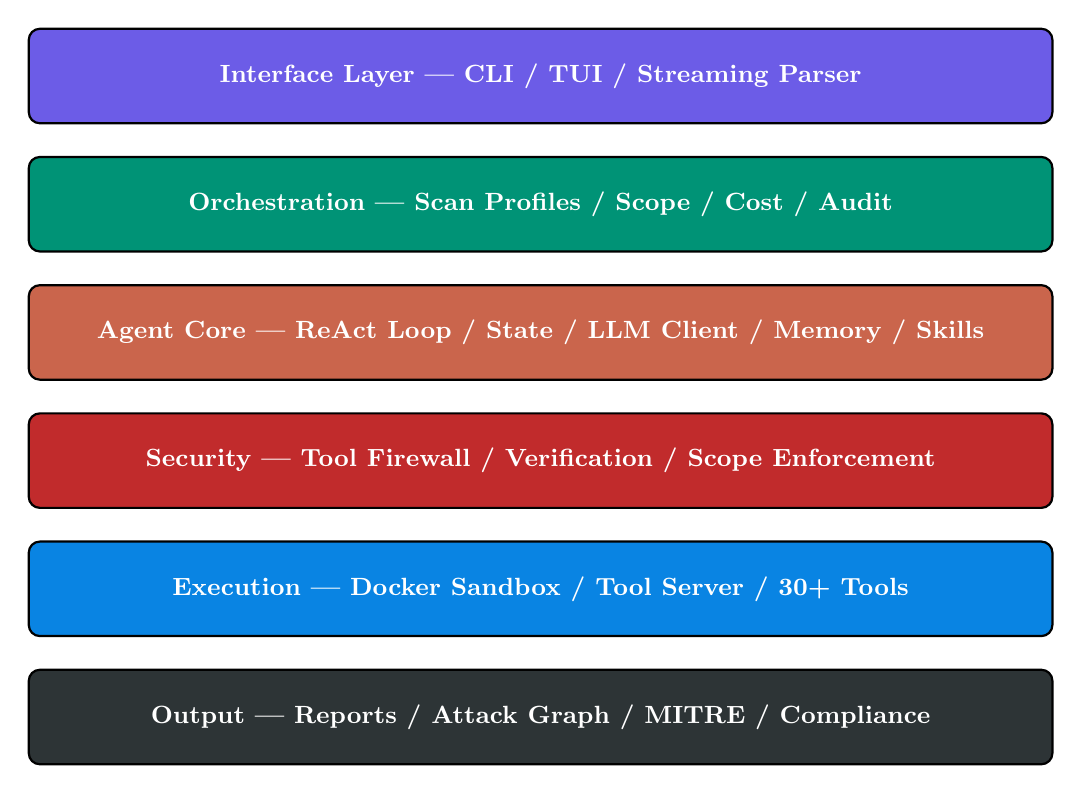
\begin{tikzpicture}[
    layer/.style={rectangle, rounded corners=4pt, minimum width=13cm, minimum height=1.2cm, draw, thick, font=\small\bfseries, text=white},
    node distance=0.4cm,
]
\node[layer, fill=phantom]       (iface)   at (0,0)   {Interface Layer --- CLI / TUI / Streaming Parser};
\node[layer, fill=green!80!black]  (orch)    [below=of iface]  {Orchestration --- Scan Profiles / Scope / Cost / Audit};
\node[layer, fill=orange!90!black] (agent)   [below=of orch]   {Agent Core --- ReAct Loop / State / LLM Client / Memory / Skills};
\node[layer, fill=red!90!black]    (sec)     [below=of agent]  {Security --- Tool Firewall / Verification / Scope Enforcement};
\node[layer, fill=blue]            (exec)    [below=of sec]    {Execution --- Docker Sandbox / Tool Server / 30+ Tools};
\node[layer, fill=dark]            (output)  [below=of exec]   {Output --- Reports / Attack Graph / MITRE / Compliance};
\end{tikzpicture}
\caption{Six-layer system architecture.}
\label{fig:layers}
\end{figure}

\section{Component Interaction}

\begin{figure}[H]
\centering
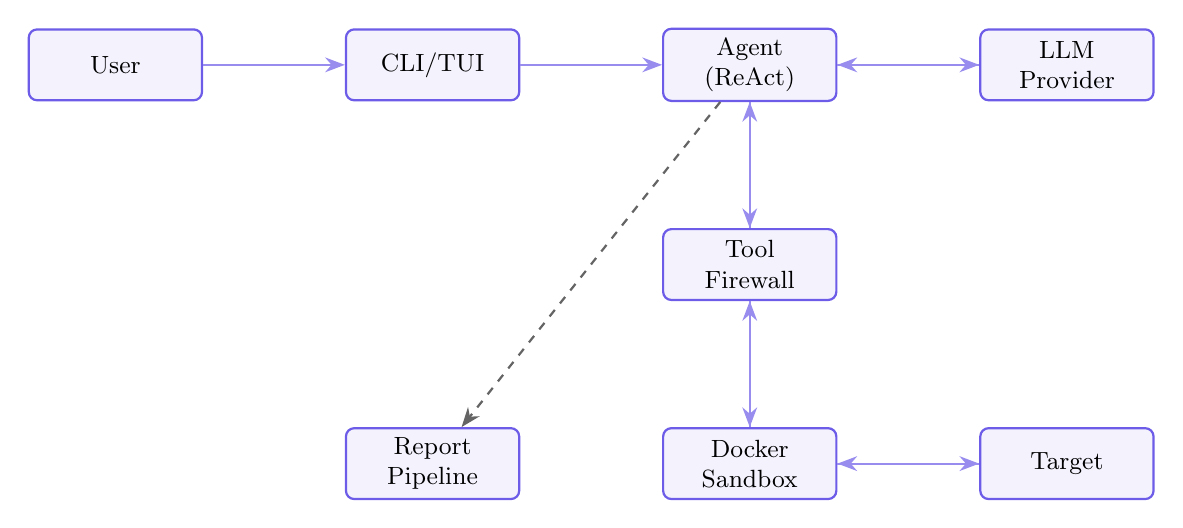
\begin{tikzpicture}[
    box/.style={rectangle, rounded corners=3pt, draw=phantom, thick, fill=phantom!8, minimum width=2.2cm, minimum height=0.9cm, font=\small, align=center},
    arr/.style={-{Stealth[length=2.5mm]}, thick, phantom!70},
    darr/.style={-{Stealth[length=2.5mm]}, thick, dashed, gray},
    node distance=1.6cm and 1.8cm,
]
\node[box] (user)    {User};
\node[box, right=of user]    (cli)     {CLI/TUI};
\node[box, right=of cli]     (agent)   {Agent\\(ReAct)};
\node[box, right=of agent]   (llm)     {LLM\\Provider};
\node[box, below=of agent]   (fw)      {Tool\\Firewall};
\node[box, below=of fw]      (sandbox) {Docker\\Sandbox};
\node[box, right=of sandbox] (target)  {Target};
\node[box, left=of sandbox]  (report)  {Report\\Pipeline};

\draw[arr] (user) -- (cli);
\draw[arr] (cli) -- (agent);
\draw[arr] (agent) -- (llm);
\draw[arr] (llm) -- (agent);
\draw[arr] (agent) -- (fw);
\draw[arr] (fw) -- (sandbox);
\draw[arr] (sandbox) -- (target);
\draw[arr] (target) -- (sandbox);
\draw[arr] (sandbox) -- (fw);
\draw[arr] (fw) -- (agent);
\draw[darr] (agent) -- (report);
\end{tikzpicture}
\caption{Data flow during a scan.}
\label{fig:dataflow}
\end{figure}

\section{Technology Stack}

\begin{table}[H]
\centering
\caption{Core technology stack.}
\begin{tabularx}{\textwidth}{lX}
\toprule
\textbf{Component} & \textbf{Technology} \\
\midrule
Language & Python 3.12+ \\
LLM Gateway & LiteLLM (100+ providers: OpenAI, Anthropic, Google, Groq, DeepSeek, Ollama, etc.) \\
Sandbox & Docker (Kali Linux base, $\sim$14\,GB, 30+ offensive tools) \\
Graph Analysis & NetworkX (attack path modeling, risk propagation) \\
Browser Testing & Playwright + Chromium (headless) \\
CLI/TUI & Click + Textual \\
Data Models & Pydantic v2 (strict validation) \\
Testing & pytest (808+ tests) \\
CI/CD & GitHub Actions (multi-platform: Linux, Windows, macOS) \\
Distribution & PyPI (\texttt{pip install phantom-agent}) + Docker + PyInstaller binaries \\
\bottomrule
\end{tabularx}
\end{table}


% ======================================================================
%  CHAPTER 3 — AGENT CORE
% ======================================================================
\chapter{Agent Core}

\section{The ReAct Reasoning Pattern}

Phantom uses the ReAct (Reasoning + Acting) paradigm, where the agent alternates between thinking about observations and taking actions.

\begin{figure}[H]
\centering
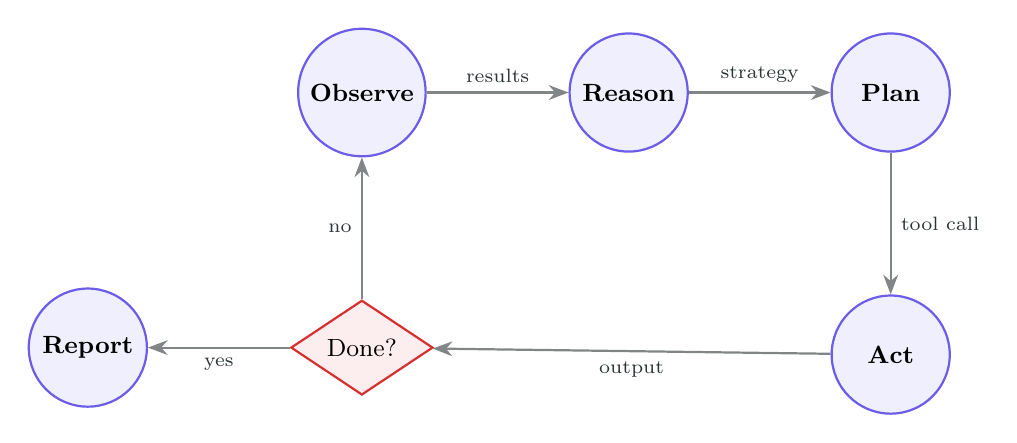
\begin{tikzpicture}[
    state/.style={circle, draw=phantom, thick, fill=phantom!10, minimum size=1.5cm, font=\small\bfseries, align=center},
    decision/.style={diamond, draw=red, thick, fill=red!8, minimum size=1cm, font=\small, align=center, aspect=1.5},
    arr/.style={-{Stealth[length=2.5mm]}, thick, dark!60},
    lbl/.style={font=\scriptsize, dark},
    node distance=1.8cm,
]
\node[state] (observe) {Observe};
\node[state, right=of observe] (reason) {Reason};
\node[state, right=of reason] (plan) {Plan};
\node[state, below=of plan] (act) {Act};
\node[decision, below=of observe] (check) {Done?};
\node[state, left=of check] (report) {Report};

\draw[arr] (observe) -- node[above, lbl] {results} (reason);
\draw[arr] (reason)  -- node[above, lbl] {strategy} (plan);
\draw[arr] (plan)    -- node[right, lbl] {tool call} (act);
\draw[arr] (act)     -- node[below, lbl] {output} (check);
\draw[arr] (check)   -- node[left, lbl] {no} (observe);
\draw[arr] (check)   -- node[below, lbl] {yes} (report);
\end{tikzpicture}
\caption{The ReAct reasoning cycle.}
\end{figure}

Each iteration: the agent receives tool output $\rightarrow$ the LLM analyzes context and plans $\rightarrow$ selects a tool with arguments $\rightarrow$ the tool firewall validates $\rightarrow$ the sandbox executes $\rightarrow$ results recorded $\rightarrow$ stop conditions checked.

\section{State Management}

Each agent maintains a bounded state (\texttt{AgentState}) tracking:
\begin{itemize}
    \item Agent ID, name, iteration count, max iterations
    \item Task description and parent agent reference
    \item Bounded conversation history with compression
    \item Start time and wall-clock limit (default: 4 hours)
\end{itemize}

The \texttt{EnhancedAgentState} extends this with vulnerability tracking, endpoint coverage, host discovery, and scan phase management. State is checkpointed every 10 iterations for crash recovery.

\section{Multi-Agent Delegation}

The root agent can spawn specialized sub-agents for focused work. Each sub-agent:
\begin{itemize}
    \item Receives a focused task (e.g., ``test SQL injection on /api/v2 endpoints'')
    \item Has its own state, conversation history, and iteration budget
    \item Shares the Docker sandbox session
    \item Returns structured results to the parent
\end{itemize}

Inter-agent messages are sanitized (XML tags, code blocks, tool-call patterns, prompt injection patterns stripped) to prevent cross-agent prompt injection.

\section{Memory Compression}

When the conversation exceeds the memory threshold (configurable per scan profile), compression is triggered:

\begin{enumerate}
    \item Older messages are chunked (10 at a time) and summarized by the LLM.
    \item Critical data (payloads, URLs, anomalies) are extracted and pinned separately.
    \item The findings ledger is \textbf{always pinned} and never compressed.
    \item Recent messages ($k=12$) are kept verbatim.
    \item Compression reduces token usage by 40--60\% on long scans.
\end{enumerate}

\section{Stop Conditions}

The agent stops when any of these conditions are met:
\begin{enumerate}
    \item \textbf{LLM-initiated:} The agent calls \texttt{finish\_scan} (minimum 5 iterations + 3 tool calls required).
    \item \textbf{Iteration limit:} Profile-defined maximum reached (60--300 depending on profile).
    \item \textbf{Time limit:} Wall-clock exceeds 4 hours.
    \item \textbf{External stop:} User cancellation or cost limit exceeded.
\end{enumerate}


% ======================================================================
%  CHAPTER 4 — LLM INTEGRATION
% ======================================================================
\chapter{LLM Integration}

\section{Provider Abstraction}

Phantom uses LiteLLM to abstract over 100+ LLM providers. Supported providers include OpenAI, Anthropic, Google Gemini, Groq (free), DeepSeek, OpenRouter, Ollama (local), and Azure.

Key features:
\begin{itemize}
    \item \textbf{Key rotation:} Comma-separated API keys with automatic rotation on rate limits.
    \item \textbf{Reasoning effort:} Configurable per scan profile (low/medium/high).
    \item \textbf{Streaming:} Token-by-token XML parsing extracts tool calls from partial responses.
\end{itemize}

\section{Cost Management}

\begin{table}[H]
\centering
\caption{Cost control mechanisms.}
\begin{tabularx}{\textwidth}{llX}
\toprule
\textbf{Control} & \textbf{Default} & \textbf{Description} \\
\midrule
Scan budget         & \$25    & Total maximum cost per scan \\
Per-request ceiling & \$5     & Maximum cost for a single LLM call \\
Input token cap     & 5M      & Cumulative input tokens \\
Output token cap    & 500K    & Cumulative output tokens \\
Compression cap     & 50      & Max memory compression LLM calls \\
\bottomrule
\end{tabularx}
\end{table}

Warning callbacks fire at 80\% and 95\% thresholds. Thread-safe via \texttt{threading.Lock}.

\section{Prompt System}

The system prompt is a 427-line Jinja2 template defining:
\begin{itemize}
    \item Agent identity, capabilities, and security rules
    \item Mandatory multi-phase methodology: Reconnaissance $\rightarrow$ Mapping $\rightarrow$ Vulnerability Testing $\rightarrow$ Exploitation $\rightarrow$ Reporting
    \item XML-based tool invocation format
    \item 20 vulnerability-specific skill files (SQLi, XSS, SSRF, IDOR, RCE, XXE, etc.) dynamically injected based on scan context
\end{itemize}


% ======================================================================
%  CHAPTER 5 — SECURITY ARCHITECTURE
% ======================================================================
\chapter{Security Architecture}

\section{7-Layer Defense Model}

\begin{table}[H]
\centering
\caption{Security layers.}
\begin{tabularx}{\textwidth}{clX}
\toprule
\textbf{\#} & \textbf{Layer} & \textbf{Function} \\
\midrule
1 & Scope Validator     & Target allowlist, DNS pinning, SSRF protection, private IP blocking \\
2 & Tool Firewall       & Argument validation, shell injection blocking, rate limiting, audit logging \\
3 & Docker Sandbox      & Ephemeral container, 4\,GB RAM, 2 CPUs, 512 PIDs, restricted capabilities \\
4 & Cost Controller     & Per-request \$5 ceiling, \$25 scan budget, token caps \\
5 & Time Limits         & Per-tool timeout (60--180s), global scan timeout (4h) \\
6 & HMAC Audit Trail    & Append-only JSONL, HMAC-signed entries, chain integrity \\
7 & Output Sanitizer    & PII stripping, API key redaction, credential scrubbing \\
\bottomrule
\end{tabularx}
\end{table}

\section{Security Audit Results}

Two deep offensive audits were performed on the codebase:

\begin{table}[H]
\centering
\caption{Security audit summary.}
\begin{tabular}{lcccc}
\toprule
\textbf{Severity} & \textbf{Found} & \textbf{Fixed} & \textbf{Verified} & \textbf{Remaining} \\
\midrule
Critical & 8 & 8 & 8 & 0 \\
High     & 19 & 19 & 19 & 0 \\
Medium   & 34 & 34 & 34 & 0 \\
Low      & 22 & 22 & 22 & 0 \\
\midrule
\textbf{Total} & \textbf{83} & \textbf{83} & \textbf{83} & \textbf{0} \\
\bottomrule
\end{tabular}
\end{table}

Notable fix categories: prompt injection defense, DNS rebinding protection, checkpoint validation, anti-premature-termination gate, HMAC audit integrity.


% ======================================================================
%  CHAPTER 6 — EXECUTION RUNTIME
% ======================================================================
\chapter{Execution Runtime}

\section{Docker Sandbox}

All offensive operations execute inside ephemeral Docker containers based on Kali Linux ($\sim$14\,GB). The container includes 30+ pre-installed security tools.

\begin{table}[H]
\centering
\caption{Sandbox specifications.}
\begin{tabularx}{\textwidth}{lX}
\toprule
\textbf{Property} & \textbf{Value} \\
\midrule
Base image       & Kali Linux (custom build: \texttt{ghcr.io/usta0x001/phantom-sandbox:latest}) \\
Memory           & 4\,GB hard limit, 6\,GB with swap \\
CPU              & 2 cores maximum \\
PIDs             & 512 (fork-bomb protection) \\
Capabilities     & \texttt{NET\_ADMIN}, \texttt{NET\_RAW} only \\
Tool server      & Port 48081, per-scan bearer token authentication \\
Lifecycle        & Created per-scan, destroyed on completion \\
\bottomrule
\end{tabularx}
\end{table}

\section{Tool Server Protocol}

The tool server is an HTTP API inside the container. Phantom sends authenticated JSON requests specifying the tool, arguments, and timeout. Output is truncated to 8\,KB to prevent context overflow.

\section{Container Lifecycle}

\begin{enumerate}
    \item \textbf{Creation:} Container started with resource limits, port mapping, environment variables.
    \item \textbf{Health check:} HTTP GET \texttt{/health} with 30 retries and exponential backoff.
    \item \textbf{Execution:} Tool calls dispatched via authenticated HTTP throughout the scan.
    \item \textbf{Cleanup:} Container stopped and removed. Port reservation released.
\end{enumerate}


% ======================================================================
%  CHAPTER 7 — TOOL ECOSYSTEM
% ======================================================================
\chapter{Tool Ecosystem}

\section{Security Tools}

\begin{table}[H]
\centering
\caption{Tool categories.}
\begin{tabularx}{\textwidth}{llX}
\toprule
\textbf{Category} & \textbf{Tools} & \textbf{Purpose} \\
\midrule
Reconnaissance & nmap, httpx, katana, whatweb & Port scanning, fingerprinting, discovery \\
Fuzzing        & ffuf, gobuster, arjun, wfuzz & Directory brute-force, parameter discovery \\
Vulnerability  & nuclei, nikto, semgrep & CVE detection, misconfiguration, code analysis \\
Exploitation   & sqlmap, commix, XSStrike & SQL injection, command injection, XSS \\
Browser        & Playwright (Chromium) & JS rendering, form interaction, SPA testing \\
Utility        & curl, python\_action, terminal\_execute & Custom scripting, API interaction \\
\bottomrule
\end{tabularx}
\end{table}

\section{Tool Integration Pattern}

Each tool follows a consistent pattern: JSON schema definition $\rightarrow$ firewall registration $\rightarrow$ execution wrapper $\rightarrow$ output parsing $\rightarrow$ result truncation (8\,KB).


% ======================================================================
%  CHAPTER 8 — REPORT PIPELINE
% ======================================================================
\chapter{Report Pipeline}

\section{7-Stage Enrichment}

Every scan runs a post-scan pipeline:

\begin{enumerate}
    \item \textbf{Verification:} Re-exploit findings with independent PoCs.
    \item \textbf{MITRE ATT\&CK:} CWE/CAPEC mapping (37 CWEs, 22 CAPECs in local database).
    \item \textbf{Compliance:} OWASP Top 10, PCI DSS v4.0, NIST 800-53 mapping with gap analysis.
    \item \textbf{Attack Graph:} NetworkX-based directed graph with path finding and risk propagation.
    \item \textbf{Nuclei Templates:} Auto-generated YAML templates for reproducible scanning.
    \item \textbf{Knowledge Store:} Cross-scan persistence updated.
    \item \textbf{Reports:} JSON, HTML, and Markdown output.
\end{enumerate}

Each stage has independent error handling --- one failure does not block subsequent stages.

\section{Output Formats}

\begin{table}[H]
\centering
\caption{Generated output files.}
\begin{tabularx}{\textwidth}{lX}
\toprule
\textbf{File} & \textbf{Purpose} \\
\midrule
\texttt{*\_report.json} & Machine-parseable, CI/CD integration \\
\texttt{*\_report.html} & Dark-theme styled report for stakeholders \\
\texttt{*\_report.md}   & Documentation, version control \\
\texttt{compliance\_report.md} & OWASP/PCI/NIST compliance posture \\
\texttt{attack\_paths.md} & Attack path analysis from graph \\
\texttt{attack\_graph.json} & NetworkX graph export \\
\texttt{vulnerabilities.csv} & Spreadsheet-compatible findings \\
\texttt{penetration\_test\_report.md} & Executive summary \\
\texttt{audit.jsonl} & HMAC-signed forensic trail \\
\bottomrule
\end{tabularx}
\end{table}


% ======================================================================
%  CHAPTER 9 — KNOWLEDGE SYSTEM
% ======================================================================
\chapter{Knowledge System}

\section{Persistent Store}

Phantom maintains a JSON-based knowledge store across scans:

\begin{itemize}
    \item \textbf{hosts.json:} Discovered hosts, ports, services, technologies.
    \item \textbf{vulnerabilities.json:} All confirmed findings with deduplication.
    \item \textbf{scan\_history.json:} Last 100 scans with metadata.
    \item \textbf{false\_positives.json:} Signatures to suppress in future scans.
\end{itemize}

Features: thread-safe via locks, atomic writes via \texttt{os.replace()}, optional Fernet encryption at rest.

\section{Checkpoint and Resume}

Agent state is checkpointed every 10 iterations. On resume (\texttt{--resume} flag), the checkpoint is loaded and the scan continues from the saved iteration. Cost controller state is preserved across resumes.


% ======================================================================
%  CHAPTER 10 — SCAN PROFILES
% ======================================================================
\chapter{Scan Profiles}

Five built-in profiles control agent behavior:

\begin{table}[H]
\centering
\caption{Scan profiles.}
\begin{tabular}{lcccl}
\toprule
\textbf{Profile} & \textbf{Iterations} & \textbf{Timeout/tool} & \textbf{Reasoning} & \textbf{Description} \\
\midrule
\texttt{quick}    & 60  & 90s  & low    & Fast, surface-level assessment \\
\texttt{standard} & 120 & 120s & medium & Balanced depth and speed \\
\texttt{deep}     & 300 & 180s & high   & Exhaustive, maximum coverage \\
\texttt{stealth}  & 60  & 60s  & medium & Low-noise, IDS/WAF evasion \\
\texttt{api\_only} & 100 & 120s & medium & API-focused, no browser \\
\bottomrule
\end{tabular}
\end{table}

Each profile defines: iteration limits, tool priority/skip lists, memory thresholds, concurrency, browser enablement, and nuclei severity filters. Profiles are consumed as natural-language constraints injected into the LLM prompt.


% ======================================================================
%  CHAPTER 11 — LIVE VALIDATION
% ======================================================================
\chapter{Live Validation}

\section{OWASP Juice Shop Scan}

A live scan was conducted against OWASP Juice Shop to validate the system:

\begin{table}[H]
\centering
\caption{Live scan configuration.}
\begin{tabularx}{\textwidth}{lX}
\toprule
\textbf{Parameter} & \textbf{Value} \\
\midrule
Target       & \texttt{http://localhost:3000} (OWASP Juice Shop v19.1.1) \\
LLM          & DeepSeek v3.2 via OpenRouter \\
Profile      & Quick (60 iterations) \\
Resume       & Yes --- interrupted at iteration 39, resumed from checkpoint at iteration 30 \\
Duration     & 27 min + 12 min = 39 min total \\
Cost         & \$0.59 + \$0.34 = \$0.93 total \\
Tool calls   & 79+ across 17 different tools \\
\bottomrule
\end{tabularx}
\end{table}

\subsection{Finding: SQL Injection --- Authentication Bypass}

\begin{infobox}[Critical Finding (CVSS 9.1)]
\begin{tabularx}{\textwidth}{lX}
\textbf{Endpoint:}  & \texttt{POST /rest/user/login} \\
\textbf{Parameter:} & \texttt{email} \\
\textbf{Payload:}   & \texttt{test@test.com' OR '1'='1'-{}-} \\
\textbf{Impact:}    & Complete authentication bypass; admin JWT obtained \\
\textbf{CWE:}       & CWE-89 (SQL Injection), CWE-287 (Improper Authentication) \\
\end{tabularx}
\end{infobox}

A working Python PoC exploit was generated demonstrating full authentication bypass and admin account takeover.

\subsection{Compliance Violations}

Violations identified: OWASP A03 (Injection), A07 (Auth Failures), PCI-DSS 6.2 (Secure Development), PCI-DSS 8.3 (Strong Auth), NIST IA-2 (Identification), NIST SI-10 (Input Validation).

\subsection{Assessment}

The scan successfully found a genuine critical vulnerability in under 40 minutes for under \$1. However, OWASP Juice Shop contains \textbf{100+ known vulnerabilities} --- Phantom found only 1 on a quick scan. This is expected for a 60-iteration budget but highlights the trade-off between speed and coverage. A deep scan (300 iterations) would provide significantly better coverage.


% ======================================================================
%  CHAPTER 12 — TESTING
% ======================================================================
\chapter{Testing and Quality Assurance}

\section{Test Suite}

808+ tests across 6 test suites:

\begin{table}[H]
\centering
\caption{Test breakdown.}
\begin{tabular}{lcc}
\toprule
\textbf{Suite} & \textbf{Tests} & \textbf{Scope} \\
\midrule
Integration (\texttt{test\_e2e\_system.py})      & 184   & Full system E2E \\
Audit fixes (\texttt{test\_v0920\_audit\_fixes.py}) & 39  & Security fix verification \\
Unit tests (\texttt{test\_all\_modules.py})       & $\sim$200 & Module-level \\
Feature tests (\texttt{test\_v0918\_features.py})  & $\sim$100 & Feature regression \\
Coverage tests (\texttt{test\_v0910\_coverage.py}) & $\sim$80  & Gap coverage \\
Security tests (\texttt{test\_security\_fixes.py}) & $\sim$50  & Security-specific \\
\midrule
\textbf{Total} & \textbf{808+} & \textbf{0 failures} \\
\bottomrule
\end{tabular}
\end{table}

\section{CI/CD}

GitHub Actions with two workflows:
\begin{itemize}
    \item \textbf{test.yml:} Runs test suite on push/PR across Python 3.12--3.13, Ubuntu/Windows/macOS.
    \item \textbf{build-release.yml:} Builds cross-platform binaries via PyInstaller on tag creation.
\end{itemize}


% ======================================================================
%  CHAPTER 13 — SYSTEM ASSESSMENT
% ======================================================================
\chapter{System Assessment}

\section{Audit Scorecard}

\begin{table}[H]
\centering
\caption{Architecture v1 audit scorecard.}
\begin{tabular}{llc}
\toprule
\textbf{Component} & \textbf{Assessment} & \textbf{Grade} \\
\midrule
Scan Profiles          & Fully implemented, 5 distinct profiles            & A$-$ \\
Memory Compression     & LLM-driven, findings pinned, production-ready     & A$-$ \\
Cost Management        & Multi-layer enforcement, thread-safe               & A \\
Report Pipeline        & 7-stage enrichment, real enrichment logic          & A$-$ \\
Attack Graph           & Real NetworkX analysis with risk propagation       & A$-$ \\
Docker Sandbox         & Solid lifecycle; gaps in cleanup and recovery      & B$+$ \\
LLM Reasoning          & Sound ReAct architecture; prompt contradictions    & B$+$ \\
Knowledge Persistence  & File-based JSON, cross-scan, encrypted             & B$+$ \\
Dynamic Stop Logic     & LLM-voluntary only; no coverage-based trigger      & C$+$ \\
\midrule
\textbf{Overall}       & \textbf{Production-beta quality}                  & \textbf{B$+$} \\
\bottomrule
\end{tabular}
\end{table}

\section{Identified Gaps}

\begin{enumerate}
    \item \textbf{System Prompt Contradictions:} The prompt simultaneously demands exhaustive scanning and efficiency. The aggressive mandate causes iteration waste.
    \item \textbf{No Coverage-Based Stopping:} No metric tracking percentage of attack surface explored. The system depends entirely on the LLM calling \texttt{finish\_scan}.
    \item \textbf{Docker Cleanup Race Condition:} The CLI signal handler has a logic bug --- sets a done flag before cleanup runs, causing container orphaning on Ctrl+C.
    \item \textbf{No Container Auto-Recovery:} If the sandbox container dies mid-scan, the scan fails. No restart or reconnect logic.
    \item \textbf{No Orphan Cleanup:} No startup scan for leftover containers from crashed runs.
    \item \textbf{Stealth Mode Advisory Only:} Rate limits and delays are injected as natural language --- the LLM could ignore them.
    \item \textbf{Stagnation Detector Not Wired:} \texttt{record\_findings\_count()} exists but is never called.
    \item \textbf{No Disk Quota:} Container has no storage limit; tools could fill host disk.
    \item \textbf{MITRE Enrichment Local-Only:} 37 CWEs is adequate for web testing but is not the full ATT\&CK database.
    \item \textbf{Single-Model Architecture:} One LLM handles everything (reasoning, compression, dedup). No model specialization.
\end{enumerate}


% ======================================================================
%  CHAPTER 14 — FIX PLAN
% ======================================================================
\chapter{Fix Plan}

\section{Priority 1: Critical Fixes}

\begin{table}[H]
\centering
\caption{Critical fixes for next release.}
\begin{tabularx}{\textwidth}{clX}
\toprule
\textbf{\#} & \textbf{Issue} & \textbf{Fix} \\
\midrule
1 & Signal handler bug & Fix CLI: call cleanup in signal handler \emph{before} setting done flag \\
2 & Scan cleanup & Move cleanup to \texttt{finally} block \\
3 & System prompt & Remove aggressive mandate; replace with coverage-guided instructions \\
4 & Wire stagnation detector & Call \texttt{record\_findings\_count()} in the agent loop \\
5 & Orphan cleanup on startup & Query Docker for stale containers and remove them \\
\bottomrule
\end{tabularx}
\end{table}

\section{Priority 2: Architecture Enhancements for v1.0}

\begin{table}[H]
\centering
\caption{Architecture enhancements.}
\begin{tabularx}{\textwidth}{clX}
\toprule
\textbf{\#} & \textbf{Feature} & \textbf{Description} \\
\midrule
6 & Coverage-based stopping & Track endpoint coverage; inject signals when coverage plateaus \\
7 & Container auto-recovery & Detect container death; recreate and resume tool server \\
8 & Stealth enforcement & Add rate-limiter middleware between agent and tool executor \\
9 & Disk quota & Add \texttt{--storage-opt size=20g} to container creation \\
10 & Capability hardening & Drop all capabilities, add back only \texttt{NET\_ADMIN}, \texttt{NET\_RAW} \\
\bottomrule
\end{tabularx}
\end{table}

\section{Priority 3: v2.0 Research Directions}

\begin{enumerate}
    \item \textbf{Model Specialization:} Cheap model for compression and dedup, expensive model for exploitation.
    \item \textbf{Reinforcement Learning:} Train tool selection from past scan outcomes.
    \item \textbf{Parallel Tool Execution:} Multiple tools from single LLM response executed concurrently.
    \item \textbf{Database Backend:} SQLite or PostgreSQL for knowledge store (team and CI use).
    \item \textbf{Real-Time Dashboard:} WebSocket-based live scan monitoring.
    \item \textbf{Vulnerability Chaining:} Automatic multi-step exploit chain construction.
    \item \textbf{Continuous Agent:} Always-on monitoring for regressions and new vulnerabilities.
\end{enumerate}


% ======================================================================
%  CHAPTER 15 — FUTURE WORK
% ======================================================================
\chapter{Future Work}

\section{Short-Term (v1.0)}

\begin{itemize}
    \item Multi-target scanning (parallel scans of multiple hosts)
    \item SARIF export for GitHub Code Scanning integration
    \item Plugin API for community tool integrations
    \item Custom scan profile creation via CLI
    \item Scan scheduling with delta reporting
\end{itemize}

\section{Medium-Term (v2.0)}

\begin{itemize}
    \item Web dashboard for scan management and visualization
    \item Collaborative multi-agent reasoning with shared memory
    \item Adaptive scan profiles based on target fingerprinting
    \item Full MITRE ATT\&CK technique-level mapping (beyond CWE/CAPEC)
    \item ISO 27001 and CIS Controls compliance frameworks
\end{itemize}

\section{Long-Term Research}

\begin{itemize}
    \item Autonomous remediation (agent-generated pull requests)
    \item Threat intelligence integration (CVE feeds, exploit databases)
    \item Red team simulation covering network, application, and social engineering
    \item Domain-specific LLM fine-tuning on pentesting datasets
\end{itemize}


% ======================================================================
%  CONCLUSION
% ======================================================================
\chapter{Conclusion}

Phantom v0.9.20 demonstrates that autonomous AI agents can conduct meaningful penetration testing with results comparable to entry-level human testers. The system successfully discovered a critical SQL injection in OWASP Juice Shop, produced a working PoC exploit, and generated compliance-ready reports --- all autonomously for under \$1 in LLM costs.

The architecture is solid at the \textbf{B+ level}: strong security controls (83 audit findings resolved), comprehensive report pipeline, real graph-based attack modeling, and production-quality cost management. The primary gaps --- system prompt contradictions, lack of coverage-based stopping, and Docker cleanup issues --- are well-understood and addressable in the next release cycle.

Architecture v1 is \textbf{functionally complete but not finished}. The core capabilities work. The 10 identified gaps require targeted fixes rather than architectural redesign. With the Priority 1 fixes applied, the system would be ready for v1.0 production release.


% ======================================================================
%  REFERENCES
% ======================================================================
\begin{thebibliography}{15}
\addcontentsline{toc}{chapter}{References}

\bibitem{react} Yao, S., et al. (2023). \textit{ReAct: Synergizing Reasoning and Acting in Language Models.} ICLR 2023.
\bibitem{owasp} OWASP Foundation (2021). \textit{OWASP Top 10 --- 2021.} \url{https://owasp.org/Top10/}
\bibitem{mitre} MITRE Corporation (2024). \textit{ATT\&CK Enterprise Matrix.} \url{https://attack.mitre.org/}
\bibitem{litellm} BerriAI (2024). \textit{LiteLLM --- Unified LLM API Gateway.} \url{https://github.com/BerriAI/litellm}
\bibitem{nuclei} ProjectDiscovery (2024). \textit{Nuclei.} \url{https://github.com/projectdiscovery/nuclei}
\bibitem{nmap} Lyon, G. (2024). \textit{Nmap --- Network Mapper.} \url{https://nmap.org/}
\bibitem{sqlmap} sqlmap developers (2024). \textit{sqlmap.} \url{https://sqlmap.org/}
\bibitem{playwright} Microsoft (2024). \textit{Playwright.} \url{https://playwright.dev/}
\bibitem{docker} Docker Inc. (2024). \textit{Docker.} \url{https://www.docker.com/}
\bibitem{pci} PCI SSC (2024). \textit{PCI DSS v4.0.} \url{https://www.pcisecuritystandards.org/}
\bibitem{nist} NIST (2020). \textit{SP 800-53 Rev.\ 5.} \url{https://csrc.nist.gov/publications/detail/sp/800-53/rev-5/final}
\bibitem{juiceshop} Kimminich, B. (2024). \textit{OWASP Juice Shop.} \url{https://owasp.org/www-project-juice-shop/}
\bibitem{networkx} Hagberg, A., et al. (2024). \textit{NetworkX.} \url{https://networkx.org/}
\bibitem{isc2} ISC$^2$ (2024). \textit{Cybersecurity Workforce Study.} \url{https://www.isc2.org/research}
\bibitem{phantom} Gadouri, R. (2026). \textit{Phantom --- GitHub Repository.} \url{https://github.com/Usta0x001/Phantom}

\end{thebibliography}

\end{document}
